\section{Example: ZX-Diagrams Optimization}

\subsection{GHZ Circuit}

We now have all the tools to simplify a ZX diagram. Notice that due to the small number of \textit{atoms}, it's way easier to come up with a complete set of rewrite rules. In contrast to the classical logic gate model, where we have many different gates, we only have two different kinds of spiders. This makes finding an efficient simplification much easier.

We will now look at a simple example of using ZX-Calculus to simplify a circuit. We will use the circuit from figure \ref{fig:ghz} as an example.

\begin{figure}
    \centering
    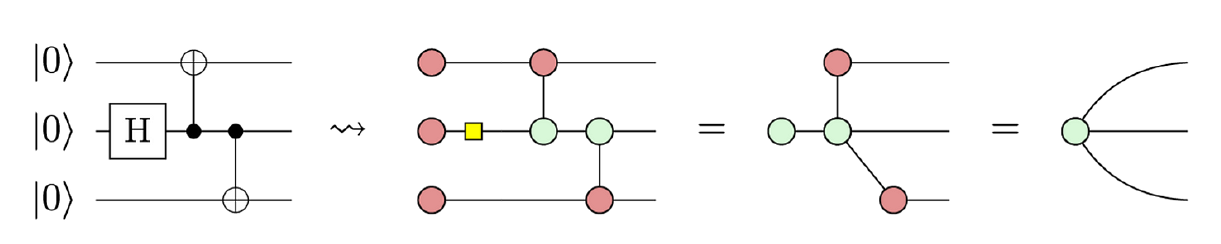
\includegraphics[width=0.45\textwidth]{images/ghz.png}
    \caption{GHZ Circuit in ZX-Calculus}
    \label{fig:ghz}
\end{figure}

To achieve a simplified circuit, we will perform these steps:

\begin{enumerate}
    \item
          In the first step, we translated the gates from the circuit into their corresponding ZX diagrams. We used the \textbf{CNOT} and \textbf{Hadamard} circuits from before to perform a lookup and translate the gates into their corresponding ZX diagrams.
    \item
          Now we can start simplifying the diagram. We will begin by applying the \textbf{Spider Fusion} rule to merge all free spiders.
    \item
          Next, we will apply the \textbf{Color Change} rule to change the color of the spider left of the Hadamard gate. This operation cancels out the Hadamard gate.
    \item
          After that, we perform the Spider Fusion rule again and remove the identity spiders; we end up with the simplified diagram shown in the rightmost diagram of figure \ref{fig:ghz}. Using the formula for calculating the matrix representation of single spiders, we compute $|GHZ\rangle = 1\cdot |000\rangle + 1\cdot |111\rangle = |000\rangle + |111\rangle$, which is proportional to the actual GHZ state. Remember that to get the correct GHZ state, we need to normalize the state first.
\end{enumerate}

By using the intermediate steps of translating the circuit into a ZX-diagram first, we were able to effortlessly calculate the matrix representation of the circuit, which would have been a lot harder if we had to calculate the matrix representation of the circuit using only its gates and the classical circuit model.

\subsection{Quantum Teleportation}

We will now look at a more complex example. We will look at the quantum teleportation circuit from figure \ref{fig:teleportation-classic}.

\begin{figure}[h]
    \centering
    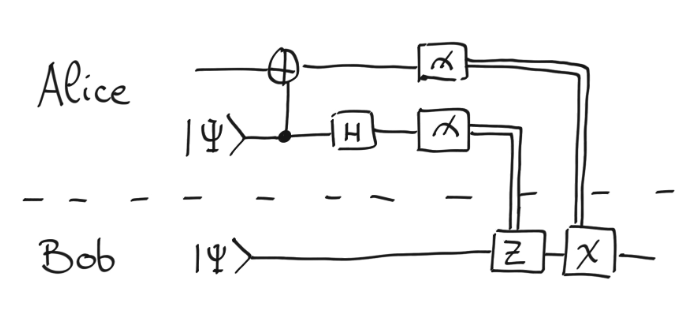
\includegraphics[width=0.45\textwidth]{images/teleportation-classic.png}
    \caption{Quantum Teleportation Circuit Img: Pennylane\cite{pennylane2023zx}}
    \label{fig:teleportation-classic}
\end{figure}

To understand the circuit, we will first look at the representation of measurements and entangled states in the ZX-Calculus.
The measurement operation in a given basis is represented by parameterized spiders of the same basis \cite{vandewetering2020zxcalculus}. The parameter of the measurement-spider is a boolean value representing the measurement outcome. Based on the measurement result, we can influence other parts of the circuit by including the parameter of the measurement spider in other spiders.
Another interesting thing to notice is that the shared bell state, which is the key to the quantum teleportation algorithm, can be represented by the spider
\zx{
    \zxNone{} \ar[d,C] \\[\zxWRow] \zxNone{}
}. This spider is the special $\eta$-morphisms we introduced earlier in the mathematical foundation of the ZX-Calculus. It has a matrix representation of
$
    \left \llbracket
    \zx{
        \zxNone{} \ar[d,C] \\[\zxWRow] \zxNone{}
    }
    \right \rrbracket =
    \begin{pmatrix}
        1 & 0 & 0 & 1 \\
    \end{pmatrix}^T = |\phi^+\rangle
$ and therefore represents a bell state.

In figure \ref{fig:teleportation}, we translated the circuit from figure \ref{fig:teleportation-classic} into a ZX diagram. Notice that it can be clearly seen from the diagram that the shared bell state works as the \textit{bridge} between Alice and Bob.

\begin{figure}[h]
    \centering
    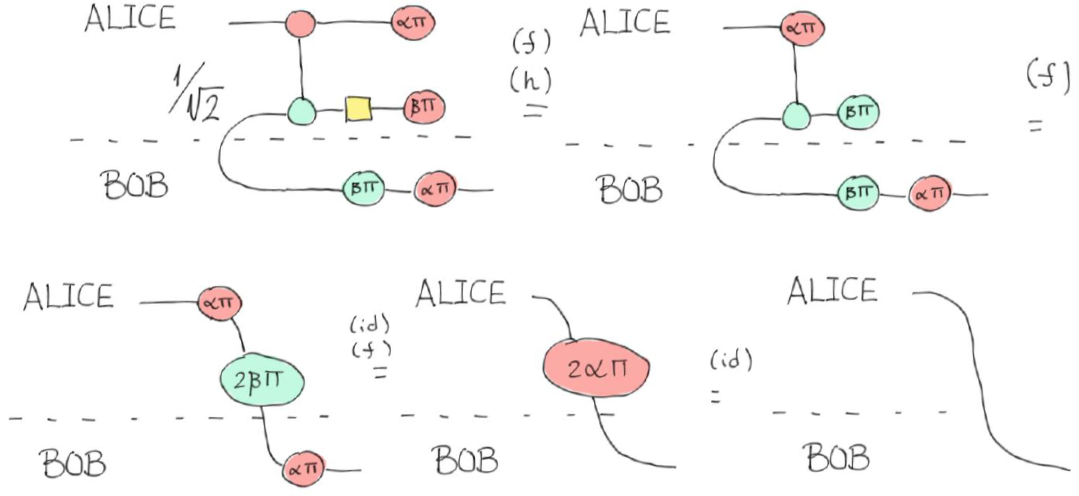
\includegraphics[width=0.45\textwidth]{images/teleportation.png}
    \caption{Teleportation in the ZX-Calculus Img: Pennylane\cite{pennylane2023zx}}
    \label{fig:teleportation}
\end{figure}

By applying the earlier rewrite rules, we can deduce that the whole circuit \textit{cancels} itself out, as the classically measured values from Alice perfectly negate the effects of Allice. This means that the circuit is equivalent to a direct channel between Alice and Bob. Therefore we showed that the teleportation works as expected.